\documentclass {report}

\usepackage[magyar]{babel}
\usepackage[utf8]{inputenc}
\usepackage{t1enc}
\usepackage{graphicx}
\graphicspath{ {Pictures/} }

\begin{document}
\title{Egylépéses gyártási feladatok költség optimális ütemezése időzített automatával}

\author{Vida Judit, gazdaságinformatikus Bsc.\\Témavezető: Dr. Hegyháti Máté, tudományos főmunkatárs\\Széchenyi István Egyetem}
\maketitle


\tableofcontents
\chapter{Bevezetés}
Ütemezési problémákkal az élet számos területén találkozhatunk, például hétköznapi feladatainkat is be kell osztanunk, az iskolában el kell osztani az órákat termekbe és a számítógép is ütemezi az elvégzendő folyamatait. Gyártórendszereknél jellemzően el kell osztani az adott erőforrásokat az azokon műveletet végző egységek között, így a gyártásütemezési feladatok az ütemezési problémák jelentős hányadát teszik ki. \\
A gyártásütemezés az iparra jellemző, a berendezéseken megadott idő alatt hajtanak végre műveleteket a termékeken. A végcél szempontjából az ütemezés célja lehet makespan minimalizálás vagy átviteli kapacitás (throughput) maximalizálás. Fontos a feladatokon elvégzett műveletek sorrendje, melyeknek a megadott módon kell egymást követniük.\\
Az irodalomban több lehetséges megoldó módszerről esik szó, gyártási probléma ütemezését elvégezték már többféle technika segítségével. A leggyakoribbak a MILP megoldó módszerek, melyek vegyes-egész lineáris programozáson alapulnak, de az S-gráf alapú megoldások is jellemzőek, valamint Petri-hálóval is oldottak már meg hasonló ütemezési feladatot.
Dolgozatomban egy gyártási probléma ütemezését választottam, amelyet költségfüggvénnyel kiterjesztett időzített automata használatával optimalizálok, és elemzem az eredményeket. Az időzített automata egy olyan automata, ahol órák segítségével modellezhetőek és korlátozhatóak az események.\\
Időzített automatával még nem járták körül bővebben a problémát, de érdemes vele foglalkozni, mert más problémaosztályok vizsgálata során hatékony módszernek bizonyult.\\
A feladat egy irodalmi példa, amelyben a meghatározott számú feladatot a gépek egy lépésben végzik el.
A feladat célja, hogy minél több feladatot elvégezzenek a gépek, és minél kevesebb legyen a kész termékek tárolási költsége.\\
A további megoldó módszerekkel elvégzett ütemezés eredményeiről szó esik a kapcsolódó irodalomban is, amelyeket fel tudunk használni arra, hogy az automatával elvégzett optimalizálás eredményeivel összehasonlítsuk őket. \\
Több modellt vizsgálunk meg, melyek eltérő korlátozási paraméterekkel rendelkeznek, így teszteljük az ütemezési folyamat lefutási idejét.

Dolgozatom második fejezetében az irodalmi háttérrel foglalkozom, a harmadik fejezetben részletezem a problémát, majd az időzített automatákról, a használt szoftverről és az LPTA alapú ütemezésről teszek említést. A negyedik fejezetben a teszteredményekről lesz szó, amelyeket korábbi megoldásokkal hasonlítok össze. A végén található az összefoglalás az ütemezés eredménye alapján, majd a dolgozat végére kerülnek a hivatkozások és a függelék. 


\chapter{Irodalmi áttekintés}
\section{Gyártási feladatok ütemezése}
Bármely gyártási ütemezési feladat rendelkezik közös vonásokkal, hasonló paraméterekkel, bármilyen módszert használunk a megoldáshoz. Közös bennük, hogy adottak a feladatok, a feladatokat elvégezni képes berendezések vagy eszközök, egy adott végrehajtási idő minden feladathoz, a cél pedig, hogy a kijelölt szempontok mellett megtaláljuk a lehető legjobb megoldást. Az egyes feladatok  végrehajtási ideje az az  időtartam, ami a munka elvégzéséhez szükséges, ez általában minden esetben egyedien meghatározott, tehát minden különböző feladatnak eltérő mennyiségű időre van szüksége. A feladatoknak lehet elvégzési határideje is, amit szintén figyelembe kell venni az ütemezés folyamán. Az irodalomban a feladatokat task megnevezéssel is használják, a munkát elvégző gépeket unit-ként, a termékeket pedig product-ként. \\\\
A problémákat különböző szempontok alapján lehet kategorizálni, az egyik csoportosítás alapján megkülönböztetünk sztochaikus és determinisztikus ütemezési feladatokat, ahol a sztochaikus típus azokat a problémákat jelöli, ahol a paraméterek futás közben kapnak értéket. A determinisztikus esetében az értékek előre be vannak állítva. \\
Egy másik csoportosítás szerint egy feladat a megadott paraméterek alapján lehet offline illetve online, ahol offline esetben a szükséges bemeneti adatok elérhetőek az ütemezés időpontjában, online esetben pedig a döntéseket meg kell hozni, mielőtt néhány paraméter értéke kiderülne. Az itt elemzett probléma az offline, determinisztikus feladatok körébe tartozik.\\
A különböző problémaesetek megoldhatóság szempontjából szintén kétféleképpen alakulhatnak. Ha az ütemezés nem elégít ki legalább egy korlátozást, akkor az nem megoldható (infeasible), minden egyéb esetben megoldható, tehát feasible. \\\\
A gyártási ütemezési feladatok egyik altípusa az egylépéses ütemezési probléma (single stage probléma), ahol a feladatokon egy tevékenységet kell végrehajtani, hogy azt befejezetté lehessen nyilvánítani. Az egylépéses problémák mellett vannak más gyakori típusok is, például a simple multiproduct, ahol a feladatot lineárisan több lépésben kell elvégezni, a general multiproduct, ami a simple multiproduct-hoz hasonló, de ki lehet hagyni lépéseket. A multipurpose (többcélú) problématípusban a lépéseknek nincs meghatározott sorrendje, tetszőlegesen hajthatóak végre. Megkülönböztethetjük a precedens típust, amely hasonló a többcélúhoz, de nem feltétlenül lineárisan hajtódnak végre a feladatok, és a general network típust, ahol a feladatokat az inputjaik és outputjaik alapján adják meg.\\
  
A single stage problémáknak a megoldásához néhány paraméternek adottnak kell lennie, például a gépek számának, valamint annak, hogy ezek a gépek azonosak-e. Két gép akkor tekinthető azonosnak, ha ugyanazokat a munkákat képesek elvégezni ugyanannyi idő alatt. Szükség van továbbá a feladatok számára és típusára. \\\\
Az egylépéses ütemezési problémákat további alosztályokra lehet bontani, a gépek az alábbiakban felsorolt típusúak lehetnek.
\begin{itemize}
\item \textbf{1 - Single Machine:} Egy gép elérhető, amelyen minden feladatot végre lehet hajtani. A termékeknek (feladatoknak) különböző feldolgozási ideje van. 
\item \textbf{Pm - Identical paralell machines}(Azonos párhuzamos gépek): m számú azonos gép áll rendelkezésre, amelyeken bármelyik egylépéses feladat végrehajtható.
\item \textbf{Qm - Paralell machines with different speed} (Párhuzamos gépek különböző sebességgel): Hasonló az előző pontban említett típushoz, de minden gépnek meghatározott sebessége van.
\item \textbf{Rm - Unrelated machines in paralell}(Párhuzamos független gépek): Hasonló a Single stage típushoz, de a feladatok elvégzési ideje egy-egy gépen inputként meghatározott.  
\end{itemize}

\section{Megoldó módszerek}
Vannak olyan módszerek, amelyekkel már a legtöbb problémaosztály szempontjából foglalkoztak, így egylépéses gyártásütemezési feladatokkal is. Az alábbi néhány eljárás a legnépszerűbb megoldók közé tartozik.


\subsection{MILP modellek}
  A MILP modellek, tehát a vegyes-egész lineáris programozási modellek a legelterjedtebb megoldó módszerek közé tartoznak, és több altípusuk létezik.\\
  \emph{Time discretization based - Időfelosztásos módszerek:}\\
   Az időfelosztásos modellek előnye, hogy széles skálán mozog a megoldható problémák típusa.
  A módszer alapján időpontokat és időréseket különböztetünk meg, A MILP modellek időpontos megadást használnak gyakrabban.  \\
  Az időbeosztásos típusban a feladatokhoz bináris változókat rendelnek aszerint, hogy a feladat az adott időpontban elvégzésre kerül, vagy nem. Amikor a feladat abban az időpontban megvalósul, akkor 1 lesz a bináris változó értéke, ha nem, akkor 0. Így annyi bináris változóra lesz szükség, ahány időpontot meghatároztunk. Lehetőleg minél kisebb számú időpont felvételével kell megtalálni az optimális megoldást a modell bonyolultságának csökkentése érdekében.\\\\
  $x_{tij},$ ahol t időpont, i a feladat, j a berendezés\\ X értéke akkor 1, ha t időpillanatban j berendezés elvégzi i feladatot.\\\\
 \emph{Precedencia alapú modellek:}\\
  Szintén bináris változókat használ az ütemezéshez, de az időfelosztásossal ellentétben kettőt. \\
  $Y_{ij}$ értéke 1, ha i feladatot j berendezés elvégzi\\
  $X_{iji'}$ értéke 1, ha j berendezés elvégzi i és i' feladatokat úgy, hogy i-t előbb, mint i'-t.\\
  Az x változó segítségével megállapítható i és i' feladatok egymáshoz való viszonya a gyártási sorrendben. \\\\
 Két altípust különböztetnek meg az alapján, hogy az időpontokat az optimalizálás előtt meghatározzák, ezek a Fix időpontos időfelosztásos módszerek, vagy pedig csak a feladat közben kerül meghatározásra az időpontok száma. Utóbbiakat Variable time model-eknek hívják, és a lényegük, hogy minél kevesebb bináris változóra legyen szükség. A modellekben folyamatos változókat használnak, amik meghatározzák mindegyik időponthoz tartozó feladatokat. 
 
 \subsection{S-gráf}
   Az első gráf alapú optimalizációra fejlesztett módszer a gyártásütemezés témakörében, amely nemcsak vizuálisan szemlélteti a folyamatot, de egyben egy matematikai modell is. Irányított gráfokból áll, amelynek a csomópontjai tevékenységek és az azokhoz vezető lépések, amelyeket az élek kötnek össze őket. Ezen kívül tartalmaznak ütemezési éleket, amelyek a meghozott ütemezési döntéseket modellezik.\\
   Létezik ütemezési döntések nélküli S-gráf is, ezt recept gráfnak hívják. \\
   A nyilak,  amelyek a csomópontokat kötik össze, a függőségeket reprezentálják a következő esetekben:

\subsection{Petri háló és automaták}
A Petri hálót és az automatát is gyakran alkalmazzák diszkrét esemény rendszerű modellezéshez,? és hogy kötegelt feladatok elvégzéséhez is alkalmas legyen, ki kellett egészíteni  időzítéssel ezeket a módszereket?. Hatékonyak, mivel jól szemléltetik a modellt, könnyen szimulálható a felépítése és a vezérlés, és a megfelelő felépítés mellett elkerülhetőek a hibák. Bár több előnyük is van a korábban említett népszerű megoldó módszerekhez képest, összességégben hatékonyságuk még elmarad a MILP és S-gráf alapú megoldó módszerekétől, valamint optimalizálásra nem alkalmasak, csak a feladat modellezésére. \\
Az időzített Petri háló alapja, hogy az átviteli jel késleltetés (delay) alapján jön létre. Többen is foglalkoztak a témával, Ghaeli foglalkozott a kötegelt folyamatok ütemezésével ilyen módon, Soares pedig megpróbálta kiterjeszteni a modellt, és valós idejű ütemezést mutatott be kötegelt rendszerekre Petri háló segítségével. 

\section{Az egylépéses ütemezés ábrázolása}
Az egylépéses ütemezési problémákat általában táblázat segítségével adják meg, ahol a sorokban tüntetik fel a munkákat, az oszlopokban pedig a rendelkezésre álló berendezéseket, a táblázatbeli metszéspontjaik ábrázolják az egyes munkák megfelelő berendezéseken való elvégzésének munkaidejét. Kopanos részletesen foglalkozott egylépéses ütemezéssel. \\
\begin{figure}[h]
\begin{center}
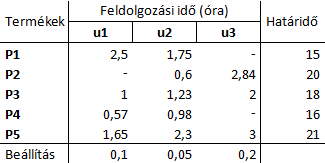
\includegraphics{tablazat1}\\
\caption{Példa egylépéses ütemezési feladat megadására.}
\end{center}
\end{figure}

A fenti ábra példa egy ütemezési feladat táblázattal való megadására, ahol a feldolgozási idő mutatja a P-vel jelölt termékek egyes gépeken való munkaidejét, a gépek u-val jelöltek. Néhány feladatot nem tud minden gép végrehajtani, ezek nem rendelkeznek feldolgozási idővel az adott gépen. \\
Minden feladathoz fel van tüntetve a hozzá tartozó határidő, valamint a gépek beállási ideje, amely a bekapcsolás után szükséges időt mutatja, amíg a gép nem tudja elkezdeni a munkát. 

\chapter{Időzített automaták}

\section{Időzített automaták}
 Egy automata eseményekből és állapotokból áll, az időzített automata pedig kiegészül órákkal, amelyek mérik a globális időt, vagy egy konkrét automata idejét. \\
 Az időzített automata a determinisztikus automaták csoportjába tartozik, ahol a determinisztikus automatákat az alábbi képlettel adják meg.
 \begin{center}
 M = (K, $\Sigma$, $\delta$, s, F)
 \end{center}
 ahol\\
 \indent \textbf{K} az állapotok halmaza\\
 \indent $\mathbf{\Sigma}$ az események véges halmaza\\
 \indent \textbf{$\delta$}: K x $\Sigma$ $\rightarrow$ K részleges átmeneti függvény\\
 \indent \textbf{s} a kezdőállapot\\
 \indent \textbf{F} az elfogadó állapotok \\
Az időzített automaták kiegészülnek órákkal, amelyek stopperóraként működnek, tehát a globálisan deklarált óra az automata teljes lefutási idejét méri.\\
Az időzített automata képlete:\\
\begin{center}
$(K, \Sigma, C, Tra, Inv, s)$\\
\end{center}
ahol\\
\indent \textbf{K} az állapotok halmaza\\
\indent $\mathbf{\Sigma}$ az események halmaza\\
\indent \textbf{C} az órák halmaza\\
\indent \textbf{Tra} K x $\phi$(C) x $ \Sigma $ x C x K időzített transitions\\
\indent \textbf{Inv} K $
\rightarrow  \phi$(C) state invariants -\\
\indent \textbf{s} a kezdőállapot \\
Az időzítést egy egyszerű szó levezetésével tudjuk bemutatni, ahol az események meghatározott időben történnek.\\
Példának vesszük az (a,1) (b,3) (a,4) (b,6) (b,10) időzített szót.\\
A fenti felírás azt mutatja, hogy melyik időpillanatban történik az esemény, amiből kiszámíthatjuk, hogy a betűk mennyi késleltetéssel követik egymást. 
\begin{center}
d1$\rightarrow$ \textbf{a} $\rightarrow$d2$\rightarrow$ \textbf{b} $\rightarrow$d1$\rightarrow$ \textbf{a} $\rightarrow$d2$\rightarrow$ \textbf{b} $\rightarrow$b4$\rightarrow$ \textbf{b}
\end{center}
ahol \emph{d} a késleltetést (delay-t) mutatja.\\
Az első \emph{a} 1 delay eltelte után kezdődhet el, és mivel \emph{b} 3 delay után következik, \emph{a}-t követően 2 delay-t kell várnia, a következő betűk pedig ennek alapján ugyanezt a szabályt követik. \\

\section{UPPAAL Cora}
A választott irodalmi példa időzített automatákkal való ütemezését az UPPAAL Cora nevű szoftver segítségével modelleztük. A szoftver alkalmas az automaták modellezésére, ütemezésére és optimalizálására meghatározott paraméterek alapján. \\
Az UPPAAL segítségével sablonokat (template-eket) hozhatunk létre, ahol minden egyes template egy különböző automata modellezésére szolgál. A sablon állapotokat és éleket tartalmaz, ahol az élek az állapotátmenetet szimbolizálják. \\
Az állapotokhoz megadhatunk nevet, illetve valamilyen korlátozást, ezen kívül beállíthatjuk az állapotát, ami initial, urgent vagy committed lehet. Az initial az automata kezdőállapotaként jelöli meg a kijelölt státuszt, a committed még inkább korlátozó, mint az urgent, tehát nem késleltetheti a következő átmenetet. Ugyanitt beállítható az is, ha az adott állapotban növekszik a költség valamely egyéb korlátozásból adódó várakozás miatt. Ekkor az állapot beállításaiban az Invariant pontban adható meg az idő előrehaladásával számított költség mértéke. \\
Az irányított élek mutatják, hogy melyik állapotból melyikbe van lehetőség átkerülni, ezen kívül pedig egyéb beállítások is megadhatóak. Minden élre megadható  Select, Guard, Sync és Update információ. A Select-ben nemdeterminisztikus választásra van lehetőség, a Guard korlátozást állít be, aminek teljesülnie kell, hogy a feladat a következő állapotba kerüljön. A Sync lehetőséggel különböző automaták állapotátmeneteit lehet összehangolni, ehhez csatorna létrehozására van szükség. Az Update segítségével frissíthetőek a változók értékei és az órák.\\
Az automata template-ek az Editor menüpont alatt helyezkednek el, és itt található még a Declarations menüpont is. 
\begin{figure}
\begin{center}
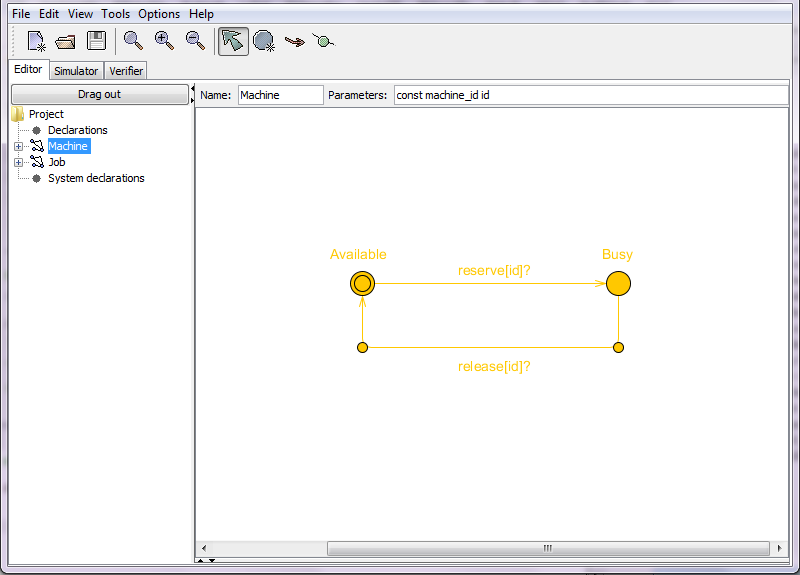
\includegraphics[width=10cm]{uppaal}
 \caption{Az UPPAAL Cora Editor ablaka}
\end{center}
\end{figure}
A  Declarations pontban az egész rendszerre vonatkozó változókat és értékeket lehet megadni, valamint függvényeket létrehozni. Az értékeket egészként kell meghatározni, mert a szoftver nem számol lebegőpontos alakban. Definiálhatunk órákat (clock), illetve csatornákat (chan), ezek az automaták közötti szinkronizálást segítik elő.\\
Minden template-hez definiálhatunk lokális változókat és paramétereket, ahol a paraméterek segítségével például meg tudjuk különböztetni a példányokat, ha a modell példányosítva van. Ekkor hozzárendelünk egy ID-t, amely sorszámot ad az automatáknak. A lokális változók között gyakran definiálunk órát, ha például egy elvégzendő feladatról van szó, külön mérhessük a munkaidejét, amit ilyenkor a modell elején le is kell nullázni.\\ 
Az Editor lapon található még a System Declarations pont, ami az automaták konkrét példányosítását végzi.\\
Az Editor mellett két fontos menüpont található. Ha nem vétettünk szintaktikai hibát, a szimulátor betölti a létrehozott automaták összes példányát, mellette pedig megjeleníti a változókat, amelyek először a kiinduló állapotban vannak, ahogy az automaták is. Itt lehetőség van egy megoldást lefuttatni, ekkor szinte biztos, hogy nem az optimális eredményt kapjuk. A lépéseket saját magunk is kiválaszthatjuk, a végeredményt pedig mindkét esetben vissza lehet játszani, vagy elmenteni egy külön fájlba.  \\
A szimulátor közben bemutatja, hogyan változtak az értékek, hogy az automaták melyik állapotukban vannak, valamint egy másik ábrán szekvencia diagramon láthatjuk a szinkronizáció lépéseit, és az automaták állapotátmenetét.\\
\begin{figure}[htpb]
\begin{center}
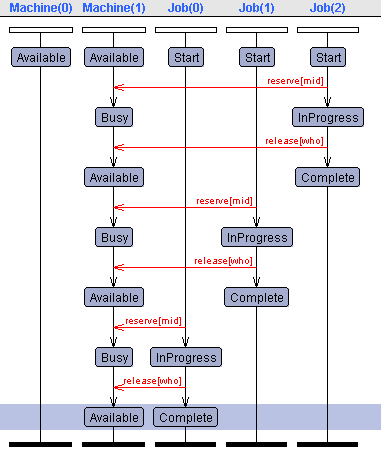
\includegraphics[height=7.5cm]{szekvencia}
\caption{A folyamat szekvenciadagramja}
\end{center}
\end{figure}
A 4.2 ábrán látható egy példa egy minta szekvenciadiagramot árázol, ahol két gépen három feladat kerül felosztásra, és bemutatja a szinkronizációs csatornák működését az egyik megoldásban.\\
A harmadik menüpont a Verifier, itt a Query-ben meg lehet adni lekérdezéseket, amelyet az UPPAAL lefuttat, majd kiírja az eredményt, amely két fajta lehet. Ha a beírt korlát alapján talált megoldást, akkor megkapjuk a \emph{Property is satisfied} üzenetet zölddel kiírva a Status pont alatt. Az Overview-nál is megjelenik a megadott Query, mellette pedig egy zöld jel. Ellenkező esetben a \emph{Property is not satisfied} üzenetet kapjuk, az Overview pedig piros jelet tesz a Query-ben megadott korlát mellé.    \\
A főmenüben leginkább az általános lehetőségeket találjuk, a Tools és az Options pontokban találhatóak egyéb beállítások az automaták ütemezésével kapcsolatban. Leellenőrizhető a Declarations és a template-ek definiálása során megadott adatok és korlátozások szintaktikai helyessége, az Options pedig az ütemezési beállításokat tartalmazza. \\
Átállítható például, hogy ütemezés során mélységi, szélességi vagy egyéb keresést alkalmazzon, valamint hasznos funkció, hogy ha a Diagnostic Trace értékét some-ra állítjuk, akkor abban az esetben, ha a Query-ben definiált lekérdezés teljesül, a megoldást be tudja tölteni a szimulátorba. A szimulátorban grafikusan, diagramon és változónként is elemezhető az eredmény. \\
Az UPPAAL Cora-hoz Java Runtime Enviroment szükséges, mivel a felhasználói interfész Java nyelven van implementálva.

\chapter{Problémadefiníció}
A probléma egy egylépéses szakaszos eljárás ütemezéséhez kapcsolódik, ahol minden termék egy termelési lépés alatt készül el, ezeket a hívjuk munkáknak. A munkákat bármelyik gép (unit) elvégezheti, de egy munka csak egy géphez rendelhető hozzá. Ugyanígy egy gép egyszerre csak egy feladaton dolgozhat, és ha már egy munkát elkezdett, azt egy másik nem előzheti meg. \\
Adott a munkák és a gépek száma, valamint a gépeknek van egy meghatározott üzembe állási ideje, ez mindegyik berendezés egyedi tulajdonsága. Két munka elvégzése között felszámolunk átállási időt, amíg a gép testre szabja saját beállításait a következő feladathoz. A gyakorlatban ez tisztítást, újra beállítást és egyéb karbantartást jelent. Az átállási időt kétféleképpen lehet megadni, az egyik típus a szekvenciafüggő, amikor a feladatok sorrendje határozza meg az értéket. Mennyiségét az szabja meg, hogy az előző és az utána következő munka között mennyi időre van szüksége a berendezésnek. A másik megadási mód a szekvenciafüggetlen típus, amikor csak a berendezéstől függ az átállási idő. Mindkét modellt be lehet állítani úgy, hogy minkét típus függjön a géptől és a feladattól is. Itt... \\
A munkákat minden gép különböző idő alatt tudja elvégezni, de olyan eset is lehet, amikor egy gép nem tudja elvégezni az adott munkát. Minden feladat rendelkezik határidővel, amit nem léphet át, miközben várakoznia kell, ha a határidő előtt elkészül. Az ütemezés célja, hogy minimalizáljuk a várakozás költségeit, emellett viszont előfordulhat, hogy a megoldás nem elégít ki a korlátozásokat, így infeasble lesz. Ha van feasible megoldás, szeretnénk lehetőleg az összes munkát elvégezni határidőre, valamint a modellt kiegészíteni korlátozásokkal úgy, hogy minél kevesebb idő alatt elvégezze az ütemezést, és minél optimálisabb eredményt adjon.  \\
A feladatban munkákat és gépeket különböztetünk meg, amelyeket később P-vel és U-val jelölünk, a product és unit szakirodalomban használt megnevezések után.

  

\chapter{Egylépéses feladat LPTA modellje}
    \section{Leírás}
    Az LPTA modell két template-ből, a rendszer deklarációkból és a változó deklarációkból áll. A template-ek egy-egy automatát írnak le, valamint saját változókkal is rendelkeznek, ezeket később részletesen be fogjuk mutatni. Ebben a példában a két sablon a gépeket és a feladatokat modellezi.\\
    A következő fejezetekben részletesen bemutatjuk a két template-et, a lekérdezéseket és a definiált paramétereket.
    \section{Template-ek és deklaráció}
    A modellben két különböző template-tel dolgozunk, ezek a Gép és Feladatok elnevezésű sémák. Mivel az ütemezést három különböző változatra bontottuk, itt az első modell kerül bemutatásra, amely nem tartalmaz korlátozásokat az ütemezési folyamat gyorsításának szempontjából.\\\\
    Az Gép elnevezésű template azt a minta gépet modellezi, amelyen a feladatokat el kell végezni. Három fő állapota van, ezek a kikapcsolt, bekapcsolt és a dolgozik. Kikapcsolt állapotból indul, és akkor kerül át bekapcsoltba, ha letelt az adott gépnek szükséges beállási idő, ezután kezdhet el dolgozni.  Ha a berendezés már bekapcsolt állapotban van, egy feladat befoglalhatja, ezt a \emph{foglal} csatorna szinkronizálja, és eltárolja, hogy melyik gép foglalt. Mielőtt \emph{Dolgozik} állapotba jutna, meg kell vizsgálnia, hogy az azon a gépen ez lesz-e az első elvégzett munka, mivel két munka elvégzése között átállási időt számol fel. Ha előtte nem dolgozott, akkor átállási idő nincs, a berendezés átvált \emph{Dolgozik} állapotba a \emph{kezdődik} csatorna segítségébel. Ellenben ha egy másik munka már megelőzte a jelenlegi munkát, az eltárolt aktuális és előző feladat azonosítója alapján ki kell várnia a hozzájuk tartozó átállási időt, és csak azután kezdheti meg a munkát. \\
    A \emph{foglal} csatorna közben szinkronizálja a gépet a feladat modelljével, a munkaidő letelte után pedig mindkét automata az \emph{elenged} csatorna segítségével jut a következő állapotba, ami a gép esetében a bekapcsolt állapot, ekkor vár az újabb feladat érkezéséig. Itt váltja át az előző munka azonosítóját, hiszen az elvégzett munka a következő lefutás során már az előző munkának fog számítani. 
    \begin{figure}[htpb]
    \begin{center}
   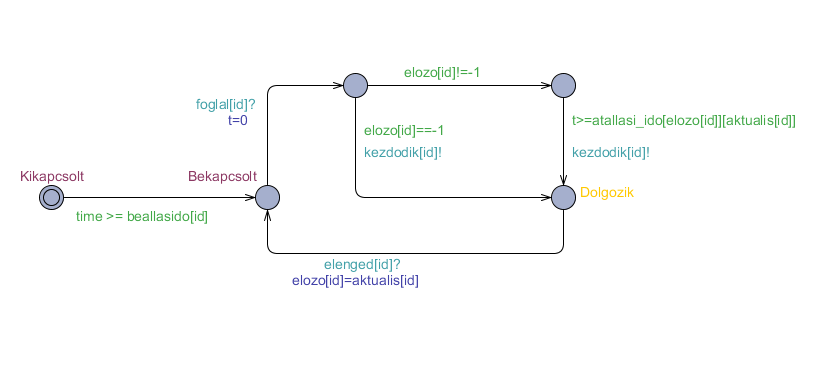
\includegraphics[width=12cm]{gep}\\
    \caption{A gép automatájának modellje}
    \end{center}
    \end{figure}\\\\\\
    A másik template a \emph{Feladatok}at mutatja be.\\
    Ez a modell öt állapotot tartalmaz, ebben az esetben a feladat a \emph{Start} stádiumból indul, ekkor a munka arra vár, hogy befoglalhasson egy gépet. Amikor ez megtörténik, átlép a \emph{Gép befoglalásra vár} elnevezésű állapotba, előtte viszont a \emph{foglal} csatorna segítségével szinkronizálja a saját státuszát a befoglalt gép státuszával, valamint elmenti, hogy aktuálisan hányas azonosító számmal rendelkező munka kerül elvégzésre ami fontos a munkaidő szempontjából, hiszem a saját magához tartozó munkaidőt kell felszámolni a gépen, és a gépnek is tudnia kell, hogy a korábban említett beállási időt meg tudja állapítani. \\
    A \emph{Gép befoglalásra vár} állapotban arra vár, hogy a befoglalt gépet beállítsák, ekkor kezdődhet el a feladat elvégzése. Minden feladathoz tartozik egy lokális óra, amelyen a munkaidejét méri, ezt a feladat kezdete előtt lenullázzuk, hogy a példányosítás során a következő feladat munkaideje ismét nullától legyen számítva. A gép beállítása után addig tartózkodik a \emph{Dolgozik} állapotban, míg a munkaideje le nem telik, ekkor újra szinkronizálja a saját és a gép státuszát, hogy a gép felszabaduljon, a feladat pedig átkerülhessen \emph{kész} állapotba. \\
    A \emph{kész} állapot azonban még nem azt jelenti, hogy a munka elkészült, hiszen a cél az, hogy pontosan a határidő leteltekor legyen leszállítva, ezért minél hamarabb készült el, annál többet kell várakoznia. Ebben a státuszban számoljuk fel a várakozás költségeit, amelyek az idő függvényében lineárisan növekednek. \\
    Amikor elérkezik a meghatározott határidő, a munka leszállításra kerül, ez a végső \emph{leszállítva} állapot.  
    \begin{figure}[htpb]
        \begin{center}
       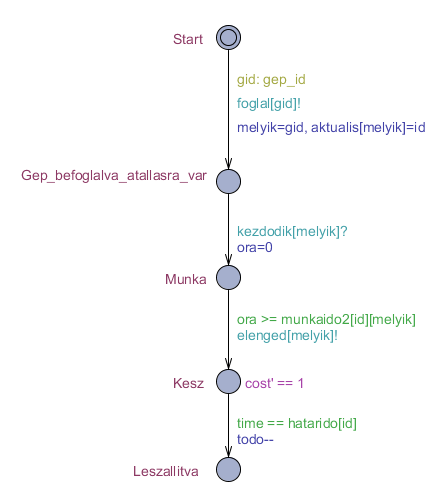
\includegraphics[height=8cm]{Feladat}\\
        \caption{A gép automatájának modellje}
        \end{center}
        \end{figure}
    \\    
    A template-ek meghatározása után a deklarációban adtuk meg a szükséges paramétereket, illetve függvényeket, amelyek szükségesek az automaták ütemezésének futtatásához. Meghatároztuk a gépek és a feladatok számát, ami az irodalmi példa szerint négy gépet és húsz feladatot jelent, majd ezeknek ki lett osztva egy saját azonosító. Szintén a globális deklarációban definiáltuk a munkaidőket gépek szerint, hiszen minden gép más-más idő alatt tud elvégezni egy feladatot. Ugyanígy megadtuk a határidőket, átállási időt, a beállási időt és a csatornákat is. Deklaráltuk a globális órát, amely a template-ektől függetlenül méri a totális időt, valamint a \emph{minTime} függvényt, ami azonban az első modellben még nem szerepel, a későbbi modellekben korlátozási céllal jelenik meg.
    \section{Lekérdezések}
    A lekérdezések segítségével adjuk meg, hogy milyen kitételt szeretnénk leellenőriztetni az ütemezés során, melyre pozitív vagy negatív válasz érkezik. A jelenlegi modellben a feltétel, amit megvizsgáltattunk az volt, hogy létezik-e olyan megoldási lehetőség, ahol minden feladat kész lesz határidőre.\\
    Hogy a lekérdezés szerkezetét leegyszerűsítsük, evezettünk a deklarációban egy változót, amelynek értéke minden esetben megegyezik a munkaszámmal. Amikor a feladat a \emph{kész} állapotból \emph{leszállítva} állapotba kerül, ezt az értéket mindig egyel csökkentjük, így optimális esetben, tehát ha minden feladat elkészül, nulla értéket vesz fel. Így a lekérdezés az alábbi módon kerül megadásra.
    \begin{center}
	\emph{E<> todo==0}
    \end{center}
    Ez a forma egyszerűbben megadható, és kiváltja a plusz változó nélküli hosszú megadást, ahol egyesével kellene ellenőrizni, hogy az adott feladat elkészült-e.
    
\chapter{Teszteredmények, összehasonlítás}
A modellt először a szükséges korlátozásokon kívül egyéb korlátozásokkal nem egészítettük ki, amikkel csökkenteni lehetett volna az ütemezés futási idejét. A Query-ben megadott cél az volt, hogy olyan megoldást találjon, amikor az összes feladatot sikeresen elvégzi, tehát leszállításra kerülnek határidőre.\\
Mivel az modellt 10 percen belül nem tudta lefuttatni az UPPAAL, az irodalmi példában szereplő 20 feladat helyett először 1 feladattal került tesztelésre az automata futási ideje, majd egyesével növeltük a feladatok számát addig, amíg a modell képes volt tíz percen belül megoldást találni rá. Az eredményeket az alábbi táblázat tartalmazza.
\begin{figure}[htpb]
\begin{center}
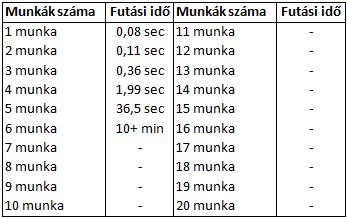
\includegraphics[height=4.4cm]{tablazat_2}
\caption{Futási eredmények korlátozás nélkül.}
\end{center}
\end{figure}

Az eredmények alapján megállapítható, hogy korlátozás nélkül a 20 munka közül csak 5 munkával futott le az ütemezés tíz percen belül, a hatodik munka hozzáadása után tíz perc alatt nem kaptunk eredményt. Emiatt a további bővítést már nem végeztük el, beláthatóan egyiknek sem lett volna eredménye belátható időn belül.





\chapter*{Hivatkozasok}
\begin{thebibliography}{99}
\bibitem Kopanos, G.M., Lainez, J.M., Puigjaner, L.: An Efficient Mixed-Integer LinearProgramming Scheduling Framework for Addressing Sequence-Dependent Setup Issues in Batch Plants. Industrial and Engineering Chemistry Research 48(13), 6346, 6357 (2009)
\bibitem Hegyháti Máté: Batch Process Scheduling: Extensions of the S-graph Framework. Doctoral School of Information Science and Technology University of Pannonia, (2015)
\end{thebibliography}

\appendix

\chapter{Jelolesek}



\end{document}
